\documentclass[12pt]{article}

% Gerald Leung, 2022.

%\usepackage{apacite}
%\usepackage[round]{natbib}
%\usepackage[colorlinks=true,linkcolor=blue]{hyperref}
\usepackage[a4paper, total={6in, 9.5in}]{geometry} % set the paper/text sizes

\usepackage{amsmath}
\usepackage{graphicx}
\usepackage[english]{babel}
\usepackage[absolute,overlay]{textpos}
\usepackage{caption}
%\captionsetup{labelformat=empty,labelsep=none}
%\captionsetup{format=hang}
%\captionsetup{font=scriptsize}
\usepackage{amssymb}
\usepackage{tcolorbox}
\usepackage{tipa}
\usepackage{siunitx}
\usepackage{adjustbox}
\usepackage{setspace}
\usepackage{lipsum}
\usepackage{physics}
\usepackage{hyperref}
\usepackage{flowchart}
\usetikzlibrary{arrows}
\usepackage{booktabs}
\usepackage{longtable}
\usepackage{layout}
\usepackage{geometry}
%\geometry{left=12mm}
\usepackage{listings}
\usepackage{xcolor}

\definecolor{codegreen}{rgb}{0,0.6,0}
\definecolor{codegray}{rgb}{0.5,0.5,0.5}
\definecolor{codepurple}{rgb}{0.58,0,0.82}
\definecolor{backcolour}{rgb}{0.95,0.95,0.92}

\lstdefinestyle{mystyle}{
    backgroundcolor=\color{backcolour},   
    commentstyle=\color{codegreen},
    keywordstyle=\color{magenta},
    numberstyle=\tiny\color{codegray},
    stringstyle=\color{codepurple},
    basicstyle=\ttfamily\footnotesize,
    breakatwhitespace=false,         
    breaklines=true,                 
    captionpos=b,                    
    keepspaces=true,                 
    numbers=left,                    
    numbersep=5pt,                  
    showspaces=false,                
    showstringspaces=false,
    showtabs=false,                  
    tabsize=2
}

\lstset{style=mystyle}


\hypersetup{colorlinks,
citecolor=blue,linkcolor=red, urlcolor=blue
}
\usepackage{qrcode}
\renewcommand{\vec}[1]{\boldsymbol{#1}}
\newcommand{\Hmns}{\tiny\textrm{H}}
\usepackage{media9}
\usepackage{aasmacros}
\usepackage{multimedia}
\usepackage{sidecap}
\usepackage{pdfpages}
\usepackage{xspace}
\usepackage{float}
%\usepackage{minted}
\usepackage{indentfirst}
\usepackage[round]{natbib}

%\usepackage[breaklinks,colorlinks,
   %urlcolor=blue,citecolor=blue,linkcolor=blue]{hyperref}
   

\newcommand{\bilby}{{\sc Bilby}\xspace}
\newcommand{\PyCBC}{{\sc PyCBC}\xspace}
\newcommand{\IPython}{{\sc IPython}\xspace}
\newcommand{\Python}{{\sc Python}\xspace}
\newcommand{\Numpy}{{\sc NumPy}\xspace}
\newcommand{\astropy}{{\sc Astropy}\xspace}
\newcommand{\R}{{\sc R}\xspace}
\newcommand{\spss}{{\sc SPSS}\xspace}


\newcommand{\be}{\begin{equation}}
\newcommand{\ee}{\end{equation}}
\newcommand{\ba}{\begin{eqnarray}}
\newcommand{\ea}{\end{eqnarray}}
\newcommand{\nn}{\nonumber}

\renewcommand{\arraystretch}{1.5}


\usepackage{etoolbox}

\makeatletter

% Patch case where name and year are separated by aysep
\patchcmd{\NAT@citex}
  {\@citea\NAT@hyper@{%
     \NAT@nmfmt{\NAT@nm}%
     \hyper@natlinkbreak{\NAT@aysep\NAT@spacechar}{\@citeb\@extra@b@citeb}%
     \NAT@date}}
  {\@citea\NAT@nmfmt{\NAT@nm}%
   \NAT@aysep\NAT@spacechar\NAT@hyper@{\NAT@date}}{}{}

% Patch case where name and year are separated by opening bracket
\patchcmd{\NAT@citex}
  {\@citea\NAT@hyper@{%
     \NAT@nmfmt{\NAT@nm}%
     \hyper@natlinkbreak{\NAT@spacechar\NAT@@open\if*#1*\else#1\NAT@spacechar\fi}%
       {\@citeb\@extra@b@citeb}%
     \NAT@date}}
  {\@citea\NAT@nmfmt{\NAT@nm}%
   \NAT@spacechar\NAT@@open\if*#1*\else#1\NAT@spacechar\fi\NAT@hyper@{\NAT@date}}
  {}{}

\makeatother


\usepackage{fancyhdr}
\fancypagestyle{CVfooter}
{
 \lhead{Gerald Leung}
 \chead{SPD Checks}
 \rhead{\today}
 \lfoot{\small{}}
 \cfoot{\small{}}
 \rfoot{\small{\thepage}}
 %\renewcommand{\headrulewidth}{0.5pt}
 %\renewcommand{\footrulewidth}{0.5pt}
}



\begin{document}
\title{Notes on Scottish Postcode Directory Quality Checking}
\author{Gerald Leung\\Public Health Scotland}
\date{Draft version: \today}
\maketitle
\tableofcontents
\section{Introduction}\label{sec:intro}
\pagestyle{CVfooter}

In this short document, we summarise the process of
the Scottish Postcode Directory (SPD) file checks from the
National Records of Scotland (NRS) by the Geospatial Team at
Public Health Scotland (PHS). In short, NRS updates
SPD files twice a year, around March and September\footnote{\url{https://www.nrscotland.gov.uk/statistics-and-data/geography/nrs-postcode-extract}}. The Geospatial Team
will then conduct quality checks of the updated files
and compare any changes with the previous version.
They will then produce lookup files in various
formats, such as \texttt{.csv}. This
document focuses on summarising the processes of quality
checking (QC)
and lookup files production using \R.
Here we also reproduce a brief summary
of the data, which can be found in Appendix \ref{appendix:dict}.
Full details can be found through the \href{https://www.nrscotland.gov.uk/files//statistics/geography/2021-2/spd-datadictionary-2021-2.pdf}{data dictionary} provided by the NRS,
or accessed through
\begin{lstlisting}
//PHIBCS/PHI/Referencing & Standards/GPD/1_Geography
/Scottish Postcode Directory/Source Data/2021_2
/ISD Data Dictionary_2021-2
\end{lstlisting}
for the \textbf{2021-2} version.

\section{Initial Quality Checks}
The \R scripts are located in 
\begin{lstlisting}
//PHIBCS/PHI/Referencing & Standards/GPD/5_GitHub/GPD/Geography
/Scottish Postcode Directory
\end{lstlisting}
and the Standard Operating Procedures (SOPs) are located in
\begin{lstlisting}
//PHIBCS/PHI/Referencing & Standards/GPD/1_Geography
/Scottish Postcode Directory/SOPs.
\end{lstlisting}
The source files can be found in
\begin{lstlisting}
//PHIBCS/PHI/Referencing & Standards/GPD/1_Geography
/Scottish Postcode Directory/Source Data.
\end{lstlisting}
They can be accessed through the organisation's VPN.
The first QC is done through the \R script \texttt{1\_Check NRS SPD.R}.

In short, this script conducts a general initial
QC of the newest version of SPD files and compares
changes with the previous version. Figure \ref{fig:block1}
shows roughly the structure of the script and the QC process.

\begin{figure}[h!]
%\centering
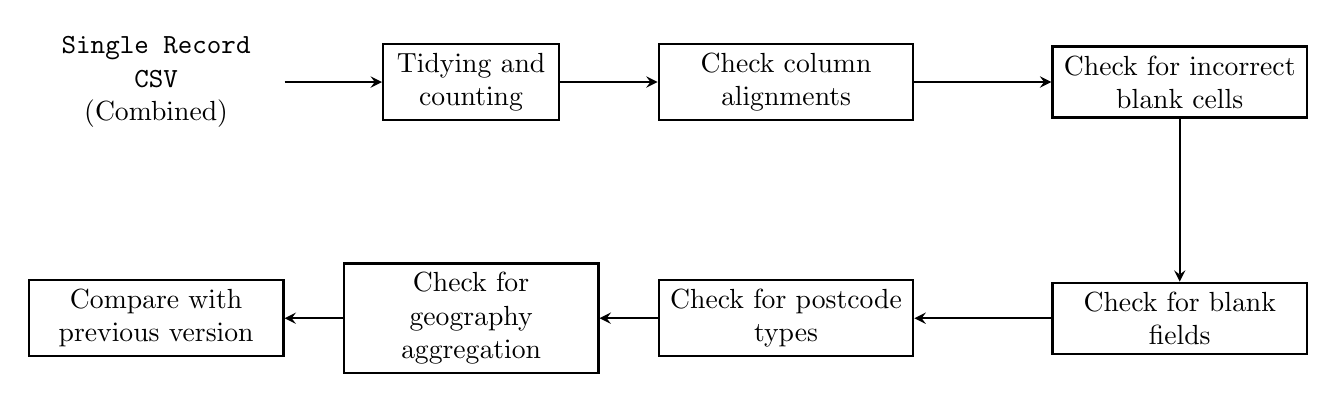
\begin{tikzpicture}[>=stealth, thick]

\node (P) at (-17,8) [text width=3cm, minimum height=0.8cm, align=flush center] 
{\texttt{Single Record CSV}\\(Combined)};

\node (A) at (-13,8) [draw, process, text width=2cm, minimum height=0.8cm, align=flush center] 
{Tidying and counting};

\node (B) at (-9,8)  [draw, process, text width=3cm, minimum height=0.8cm, align=flush center] 
{Check column alignments};


\node (B2) at (-4,8)  [draw, process, text width=3cm, minimum height=0.8cm, align=flush center] 
{Check for incorrect blank cells};

\node (B3) at (-4,5)  [draw, process, text width=3cm, minimum height=0.8cm, align=flush center] 
{Check for blank fields};

\node (B4) at (-9,5)  [draw, process, text width=3cm, minimum height=0.8cm, align=flush center] 
{Check for postcode types};

\node (B5) at (-13,5)  [draw, process, text width=3cm, minimum height=0.8cm, align=flush center] 
{Check for geography aggregation};

\node (B6) at (-17,5)  [draw, process, text width=3cm, minimum height=0.8cm, align=flush center] 
{Compare with previous version};

\draw[->] (P) -- (A);

\draw[->] (A) -- (B);
%\draw[->] (B) -- (B1);
\draw[->] (B) -- (B2);
%\draw[->] (B) -- (B3);
\draw[->] (B2) -- (B3);
\draw[->] (B3) -- (B4);
\draw[->] (B4) -- (B5);
\draw[->] (B5) -- (B6);


\end{tikzpicture}
\caption{Schematic diagram of the initial QC process.}\label{fig:block1}
\end{figure}

To start with, all empty rows contained in the files
are removed and the files are combined. The user will then
record the total number of records and postcode types (\texttt{Large User} or \texttt{Small User}).
Sanity checks are conducted to make sure there are
no blank entries for Health Board and Council Areas.
The script then checks for postcodes that moved
from Glasgow City Council to North Lanarkshire Council
(eight in total).
Checks are then carried out to make sure columns are
aligned correctly. For example, between Health Board Area
Code and Council Area Code columns to make sure their values in 1995 (e.g. \texttt{HealthBoardArea1995Code}) represent the same area in 2006 (e.g. \texttt{HealthBoardArea2006Code}). This is generally done
by assigning a number to the case when a particular
column does not have an expected code that should match
with the other column. For instance:
\begin{lstlisting}[language=R,frame=single]
HB_issue = case_when(HealthBoardArea1995Code == '01' & 
                              HealthBoardArea2006Code != 'S08000008' ~ 1)
Count(HB_issue)
\end{lstlisting} 
Refer to Appendix \ref{appendix:dict} or the NRS
data dictionary mentioned in Section \ref{sec:intro}
for more information of the data.
 
 Extensive checks are then carried
out to make sure there are no blank fields, through the \texttt{checks} function

\begin{lstlisting}[language=R,frame=single]
checks <- function(variable1, variable2){
  
  spd %>% 
    mutate(check = case_when(variable1 == "" & variable2 != "" ~ 1, 
                             variable1 != "" & variable2 == "" ~ 2)) %>% 
    count(check) %>% 
    print()
  
}
\end{lstlisting}
So for instance, we should expect that
if \texttt{OutputArea2001Code} is blank, then\\
\texttt{DataZone2001Code} should also be blank since
the data zones are made up of output areas. Throughout
the script, blank fields are also checked by, for example,

\begin{lstlisting}[language=R]
spd %>% summarise(missing = sum(is.na(DataZone2001Code)))
\end{lstlisting}
where \texttt{spd} refers to the \texttt{SingleRecord.csv}
data frame.


Examinations are also
carried out to make sure there are no English voting codes included. Some checks are also carried to make sure
there are no errors with postcodes and their
split indicators.
Finally, the script makes sure that mappings are done correctly,
such as Data Zones and Health Boards.

The script also makes comparisons with previous SPD files.
For instance,it checks for changes in postcodes
(some have been deleted), different data zones and
health boards etc.

 
\section{Lookup Files}
The next step of the process is to produce lookup files for
other uses and analysis within the organisation. This is done through the \texttt{2\_Create Postcode Lookup Files.R} script. Figure \ref{fig:block2} shows an overview of the process. To begin
with, all the variables are renamed and changed into
correct format. The Urban Rural codes are changed into
named columns. Some formatting are done to ensure
consistency with \R and \spss. For instance, by adding
leading zeros to some columns and making sure
blank cells are represented as \texttt{NA}. The script
then connects to the PHS Open Data website\footnote{\url{https://www.opendata.nhs.scot/}}   
to access Geography Codes and Names data file,
which are then used for column names, including
Data Zone, Intermediate Zone, Council Area,
Health and Social Care Partnership and Health Board.
These are then merged with the original
\texttt{SingleRecord.csv} to produce the lookup file.

\begin{figure}[h!]
%\centering

\begin{tikzpicture}[>=stealth, thick]

\node (P) at (-19,8) [text width=4cm, minimum height=0.8cm, align=flush center] 
{\texttt{SingleRecord.csv}\\(Checked)};

\node (A) at (-14.5,8) [draw, process, text width=2cm, minimum height=0.8cm, align=flush center] 
{Renaming and formatting};

\node (B) at (-10,8)  [draw, process, text width=3cm, minimum height=0.8cm, align=flush center] 
{Add column names from Open Data API};


\node (B2) at (-6,8)  [text width=2cm, minimum height=0.8cm, align=flush center] 
{SPD lookup file};


\draw[->] (P) -- (A);

\draw[->] (A) -- (B);
\draw[->] (B) -- (B2);


\end{tikzpicture}
\caption{Schematic diagram of the lookup file production process.}\label{fig:block2}
\end{figure}

\section{Updating Postcode Table}
After QC, the data needs to be uploaded to the
corporate data warehouse (CDW). The lookup files are found in
\begin{lstlisting}
//PHIBCS/PHI/Referencing & Standards/GPD/1_Geography
/Scottish Postcode Directory/Lookup Files.
\end{lstlisting} 
The tables from
the previous SPD files have to be updated to satisfy
any requirements from the IT. Some columns
are not required and therefore removed. On the other hand,
there are columns that are no longer supplied by the NRS.
They are however still required for CDW and therefore
must be added here. The columns are renamed and finally
reordered, and saved as
\begin{lstlisting}
//PHIBCS/PHI/Referencing & Standards/GPD/1_Geography
/Scottish Postcode Directory/Lookup Files
/Scottish_Postcode_Directory_2021-2_CDW.csv
\end{lstlisting} 
for the \textbf{2021-2} version.

\section{Testing Postcode Table}
The file is then uploaded to APXU by IT,
which requires testing. This is done with the script
\texttt{5\_Check Postcode table on MGSREF APXU}.
We start off by connecting to the APXU and access
the database there. 

\newgeometry{left=10mm,right=40mm}
\appendix
\section{Appendix: Data Dictionary}\label{appendix:dict}
Here we reproduced and summarised the data dictionary provided by the NRS. Table {\ref{tab:SPD_DICT}} shows the rough definition of the data within \texttt{SingleRecord.csv}
in order.

\begin{longtable}{|| m{.55\textwidth} | m{.12\textwidth} | m{.47\textwidth}||} 
\hline
\textbf{Name} & \textbf{Type} & \textbf{Notes} \\
\hline\hline
CensusHouseholdCount1991 & Integer & 1991 Census postcode usually resident household count.\\ \hline
CensusHouseholdCount2001 & Integer & 2001 Census postcode household count.\\ \hline
CensusHouseholdCount2011 & Integer & 2011 Census postcode household count.\\ \hline
CensusPopulationCount1991 & Integer & 1991 Census postcode residential count.\\ \hline
CensusPopulationCount2001 & Integer & 2001 Census postcode residential count.\\ \hline
CensusPopulationCount2011 & Integer & 2011 Census postcode residential count.\\ \hline
CivilParish1930Code & Character & 1930 Civil Parish code.\\ \hline
CommunityHealthPartnership2004Code & Character & 2004 Community Health Partnership code \textbf{\textit{(ISD version only)}}.\\ \hline
CommunityHealthPartnership2007Code & Character & 2007 Community Health Partnership code \textbf{\textit{(ISD version only)}}.\\ \hline
CommunityHealthPartnership2011Code & Character & 2011 Community Health Partnership code \textbf{\textit{(ISD version only)}}.\\ \hline
CommunityHealthPartnership2012Code & Character & 2012 Community Health Partnership code \textbf{\textit{(ISD version only)}}.\\ \hline
CommunityHealthPartnershipSubAreas2011Code & Character & 2011 Community Health Partnership sub sector code \textbf{\textit{(ISD version only)}}.\\ \hline
CouncilArea2011Code & Character & 2011 Council Area code \textbf{\textit{(ISD version only)}}.\\ \hline
CouncilArea2018Code & Character & 2018 Council Area code \textbf{\textit{(ISD version only)}}.\\ \hline
CouncilArea2019Code & Character & 2019 Council Area code.\\ \hline
DataZone2001Code & Character & 2001 Data Zone built from 2001 Output Areas.\\ \hline
DataZone2011Code & Character & 2011 Data Zone built from 2011 Output Areas.\\ \hline
DateOfIntroduction & Date & Postcode introduction date. Currently shown as $\#\#\#\#$ on the \texttt{csv} file. \\ \hline
DateOfDeletion & Date & Postcode deletion date.
Similarly to date of introduction. \\ \hline
DeliveryPointCount & Integer & The Royal Mail delivery point count.\\ \hline
DeliveryPointCountNonResidential & Integer & Non-residential delivery point count.\\ \hline
ElectoralWard2019Code & Character & 2019 Electoral Ward code.\\ \hline
EnterpriseRegion2008Code & Character & 2008 Scottish Enterprise Region code.\\ \hline
GridLinkIndicator & Character & Whether grid reference has been assigned via GridLink (Y/N).\\ \hline
GridLinkPositionalAccuracy & Character & Positional accuracy of the GridLink grid reference allocated to each postcode. See full dictionary for details.\\ \hline
GridReferenceEasting & Character & Grid reference easting.\\ \hline
GridReferenceNorthing & Character & Grid reference northing.\\ \hline
HealthBoardArea1995Code & Character & 1995 Health Board code.\\ \hline
HealthBoardArea2006Code & Character & 2006 Health Board code.\\ \hline
HealthBoardArea2014Code & Character & 2014 Health Board code \textbf{\textit{(ISD version only)}}.\\ \hline
HealthBoardArea2018Code & Character & 2018 Health Board code \textbf{\textit{(ISD version only)}}.\\ \hline
HealthBoardArea2019Code & Character & 2019 Health Board code.\\ \hline
HouseholdCount & Integer & The Royal Mail Household count.\\ \hline
Imputed & Character & Whether postcode's higher area values
have been inputed \textbf{\textit{(ISD version only)}}.\\ \hline
IntegrationAuthority2016Code & Character & 2016 Integration Authority code (Health and Social Care Partnership) \textbf{\textit{(ISD version only)}}.\\ \hline
IntegrationAuthority2018Code & Character & 2018 Integration Authority code (Health and Social Care Partnership) \textbf{\textit{(ISD version only)}}.\\ \hline
IntegrationAuthority2019Code & Character & 2019 Health and Social Care Partnership code.\\ \hline
IntermediateZone2001Code & Character & 2001 Intermediate Zone built from 2001 Data Zones.\\ \hline
IntermediateZone2011Code & Character & 2011 Intermediate Zone built from 2011 Data Zones.\\ \hline
Islands2021Code & Character & Island identification code.\\ \hline
Latitude & Numeric & Coordinates in degrees.\\ \hline
Longitude & Numeric & Coordinates in degrees.\\ \hline
LAU2019Level1Code & Character & European Area Classification Local Administrative Unit (LAU) 2019 level 1. E.g. Council areas.\\ \hline
LinkedSmallUserPostcode & Character & Small User postcode that
contains the grid reference of the Large User postcode.\\ \hline
LinkedSmallUserPostcodeSplitChar & Character & Split indicator for small user, A, B, C \textbf{\textit{(ISD version only)}}.\\ \hline
Locality1991Code & Character & 1991 Locality code.\\ \hline
Locality2001Code & Character & 2001 Locality code.\\ \hline
Locality2016Code & Character & 2016 Locality code.\\ \hline
LocalGovernmentDistrict1991Code & Character & 1991 Local Government District code.\\ \hline
LocalGovernmentDistrict1995Code & Character & 1995 Local Government District code.\\ \hline
NationalPark2010Code & Character & 2010 National Park code.\\ \hline
NeverDigitised & Character & Whether a postcode boundary has been digitised (Y/N).\\ \hline
NUTS2018Level2Code & Character & European Area Classification Nomenclature of Territorial Units for Statistics (NUTS) 2018 level 2.\\ \hline
NUTS2018Level3Code & Character & European Area Classification Nomenclature of Territorial Units for Statistics (NUTS) 2018 level 3.\\ \hline
OutputArea1991Code & Character & 1991 Census Output Area code.\\ \hline
OutputArea2001Code & Character & 2001 Census Output Area code.\\ \hline
OutputArea2011Code & Character & 2011 Census Output Area code.\\ \hline
Postcode & Character & The Royal Mail postcode. Consists of area, district, sector and unit. E.g. AB1 0AA.\\ \hline
PostcodeDistrict & Character & Postcode District. E.g. AB1. \\ \hline
PostcodeSector & Character & Postcode Sector. E.g. AB1 0.\\ \hline
PostcodeType & Character & Small (S) or Large (L) \textbf{\textit{(ISD version only)}}.\\ \hline
RegistrationDistrict2007Code & Character & 2019 Council Area (same as Council Area boundaries).\\ \hline
ROACommunityPlanningPartnership2006Code & Character & 2006 Regeneration Outcome Area Community Planning Partnerships (CPP) code.\\ \hline
ROALocal2006Code & Character & 2006 Regeneration Outcome Area Local code.\\ \hline
Settlement2001Code & Character & 2001 Settlement code.\\ \hline
Settlement2016Code & Character & 2016 Settlement code.\\ \hline
ScottishIndexOfMultipleDeprivation2020Rank & Character & Rank Data Zones (2011) according to deprivation.\\ \hline
ScottishParliamentaryRegion2021Code & Character & 2021 Scottish Parliamentary Region code.\\ \hline
ScottishParliamentaryConstituency2021Code & Character & 2021 Scottish Parliamentary Constituency code.\\ \hline
SplitChar & Character & Split indicator A, B, C \textbf{\textit{(ISD version only)}}. \\ \hline
SplitIndicator & Character & Split postcode indicator. Y/N.\\ \hline
StrategicDevelopmentPlanningArea2013Code & Character & 2013 Strategic Development Planning Area code.\\ \hline
TravelToWorkArea2011Code & Character & 2011 Travel to Work Area code.\\ \hline
UKParliamentaryConstituency2005Code & Character & 2005 UK Parliamentary Constituency code.\\ \hline
UrbanRural2Fold2016Code & Character & Standard definition of rural Scotland following the Scottish Government Urban Rural classification (2 fold) \textbf{\textit{(ISD version only)}}.\\ \hline
UrbanRural3Fold2016Code & Character & Similarly to above (3 fold) \textbf{\textit{(ISD version only)}}.\\ \hline
UrbanRural6Fold2016Code & Character & Standard definition of rural Scotland following the Scottish Government Urban Rural classification (6 fold).\\ \hline
UrbanRural8Fold2016Code & Character & Similarly to above (8 fold).\\ \hline



\caption{Data dictionary of the SPD file. Reproduced from NRS.} % needs to go inside longtable environment
\label{tab:SPD_DICT}
\end{longtable}
%\restoregeometry
%\end{table} 


%\bibliographystyle{ieeetr}
%\bibliographystyle{yahapj}
%\bibliography{slidescites}


\end{document}